\section{Theorie}
Es ist bekannt, dass Metalle eine gut elektrische Leitfähigkeit haben. Dies liegt an der gitterartigen Struktur der Metallatome.
Die Leistungselektronen können sich im Metallinneren frei bewegen, da fast alle Atome ionisiert sind. Im Inneren herrscht gegenüber dem
Außenraum ein Potential $\Phi$.
Dieses kann als ein Potentialtopf-Modell angesehen werden, was in Abbildung \ref{abb:1} schematisch
dargestellt ist. Wenn ein Elektron aus diesem Potential austritt, muss
es die Austrittsarbeit $e_0 \Phi$ aufbringen. Dabei ist $e_0$ die Elementarladung.
\begin{figure}[H]
  \centering
  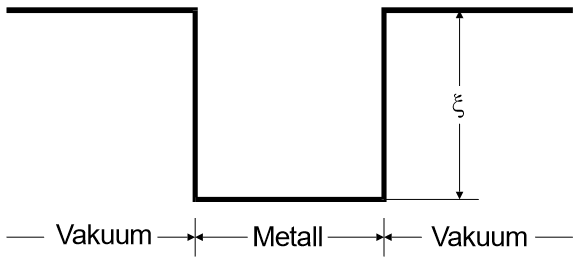
\includegraphics[width=5 cm, height= 2.5cm]{content/Potentialtopf.png}
  \caption{Potentialtopf-Modell \cite{1}.}
  \label{abb:1}
\end{figure}
Um Messungen durchführen zu können, muss zunächst die Apparatur näher erläutert werden.
Es handelt sich, wie in  Abbildung \ref{abb:2} zu sehen ist, um eine Hochvakuum-Diode.
\begin{figure}[H]
  \centering
  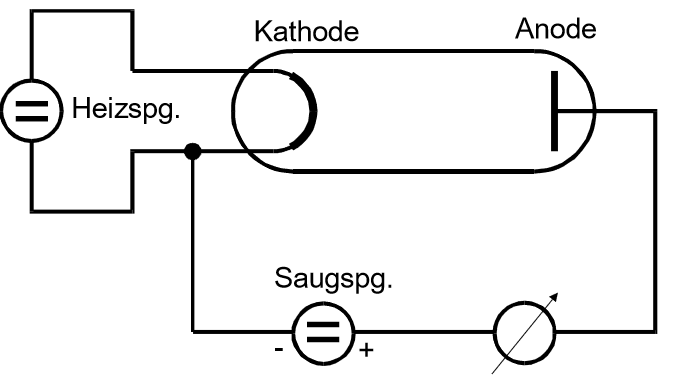
\includegraphics[width=10 cm, height =5cm]{content/Aufbau.png}
  \caption{Darstellung einer Vakuum-Diode \cite{1}.}
  \label{abb:2}
\end{figure}
An der Kathode werden die Elektronen durch den Heizstrom emittiert und mit einer Saugspannung zur
Anode beschleunigt. Sie ist deshalb evakuiert, da sonst die freien Elektronen mit den Gasmolekülen wechselwirken.
Eine typische Kennlinie zwischen Strom und Spannung ist in Abbildung \ref{abb:3} dargestellt.
\begin{figure}[H]
  \centering
  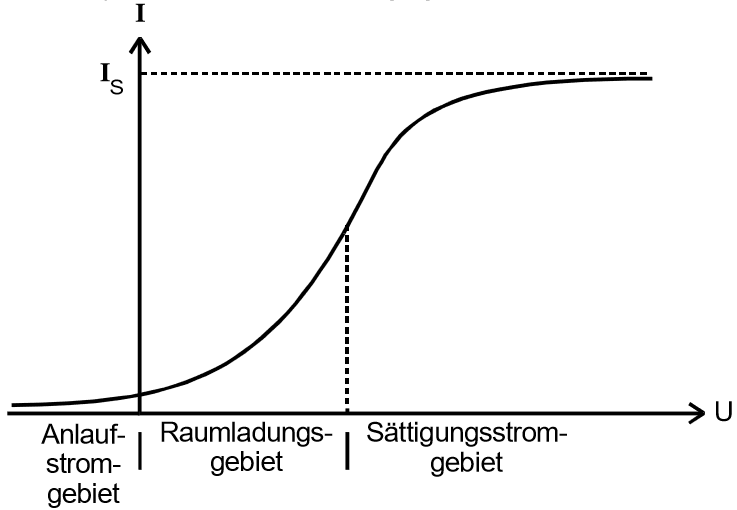
\includegraphics[width=10 cm , height= 5 cm]{content/Kennlinie.png}
  \caption{Kennlinie einer Vakuum-Diode \cite{1}.}
  \label{abb:3}
\end{figure}
Dabei beschreibt $I_s$ den Sättigungsstrom von den erzeugten Elektronen.
Im folgenden werden die drei Gebiete näher erläutert.\\
Das \textbf{Anlaufstromgebiet} zeigt bei einer negativer Spannung ein minimalen Stromfluss. Dies lässt sich auf die
statistisch verteilte Eigengeschwindigkeit der Elektronen zurückführen. Es erreichen trotz Gegenspannung
einige Elektronen, die mit mit einer endlichen Geschwindigkeit aus dem Metall austreten, die Anode.
Der Zusammenhang zwischen der Anlaufstromstärke und der Spannung ist gegeben durch
\begin{equation}
  j(V) = \text{const} \cdot \exp\left(\frac{-e_0 V}{k_b T}\right).
  \label{eq:1}
\end{equation}
Dabei ist $V$ die Spannung, $T$ die Temperatur und $k_b$ die Bolzmann-Konstante.\\
Im \textbf{Raumladungsgebiet} erreichen nicht alle emittierten Elektronen die Anode.
Dies liegt daran, dass die Geschwindigkeit $v$ der frei erzeugten Elektronen nicht konstant ist. Das hat zur
Konsequenz, dass die Raumladungsdichte $\rho$ eine Funktion des Ortes ist. Sie nimmt zur Anode hin ab.
Die Stromdichte $j$ ist gegeben durch:
\begin{equation*}
  j = -\rho v
\end{equation*}
Die Proportionalität von Strom und Spannung, die durch das
Ohmsche Gesetz gegeben ist, gilt in diesem Fall nicht. Der Zusammenhang lässt sich in diesem Fall mit der Langmuir-Schottkyschen Raumladungsgleichung
beschreiben
\begin{equation}
  j = \frac{4}{9} \epsilon_0 \sqrt{2\frac{e_0}{m_0}} \frac{V^\frac{3}{2}}{a^2}.
  \label{eq:2}
\end{equation}
Dabei beschreibt $a$ den Abstand zwischen Kathode und Anode und $m_0$ die Masse des Elektrons.\\
Anschließend folgt das \textbf{Sättigungsstromgebiet}. Dieses Gebiet beschreibt die Zahl der Elektronen, die pro
Zeit- und Flächeneinheit aus der Metalloberfläche in Abhängigkeit der Temperatur austreten.
Die Elektronen erreichen alle die Anode und sind nur von der Austrittsarbeit $e_0 \cdot \Phi$ und Temperatur $T$
abhängig.
Durch die Integration über jedes kleine Flächenelement ergibt sich die Richardson-Gleichung
\begin{equation}
  j(T) = 4 \pi \frac{e_0 m_0 k_b^2}{h^3} T^2 \exp\left(\frac{-e_0 \Phi}{k_bT}\right).
  \label{eq:3}
\end{equation}
Dabei ist $h$ das Plancksche Wirkungsquantum.
